\begin{block}{Gene Regulatory Network Model}
\vspace{-1ex}
\begin{figure}
    \centering
    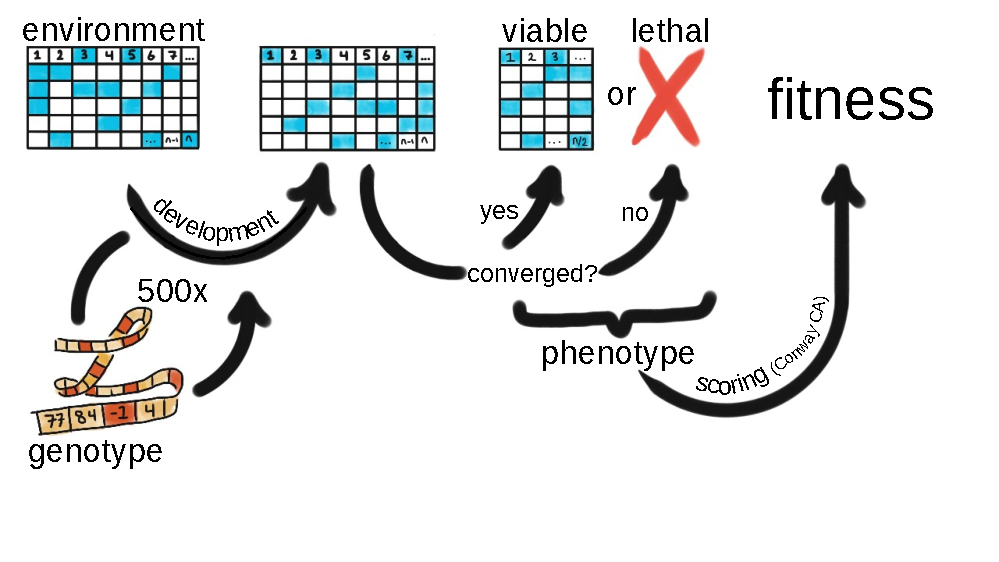
\includegraphics[width=0.8\textwidth,trim={0 1.5cm 0 0.25cm},clip]{img/complete_schematic}
 	%\captionsetup{singlelinecheck=off,justification=raggedright}
  	\caption{A cartoon overview of the development and assessment processes of the expanded model, based loosely on \cite{Wilder2015ReconcilingEvolvability}.}
    \label{fig:complete_schematic}
\end{figure}
{\small 
A genome consists of a fixed-length set of if-then rules.
Each rule has three components: the index of a chemical antecedent, the index of a chemical patient, and description of the action of the antecedent on the patient.
This relationship may be inhibitory, excitatory, or neutral.
To generate the phenotype, the genomic rules are applied 500 times to an initial state $S(0)$, representing the environment, yielding a final state $S(500)$.
A phenotype is deemed inviable if $S(500) \neq S(501)$.
To enable sophisticated regulatory interactions in the network, viable phenotypes are defined as a subset of the final set of chemical states $S(500)$ so that a portion of chemical products are hidden from direct exposure in the phenotype.
Phenotypic fitness is assessed using a metric based on Conway's cellular automata.
}
\end{block}
